A raised crosswalk (\figref{xwalk}) is a designated street crossing that simulatneously acts as a speed hump by bringing the level of the roadway to that of the sidewalk.

\begin{figure}[h]
	\centering
	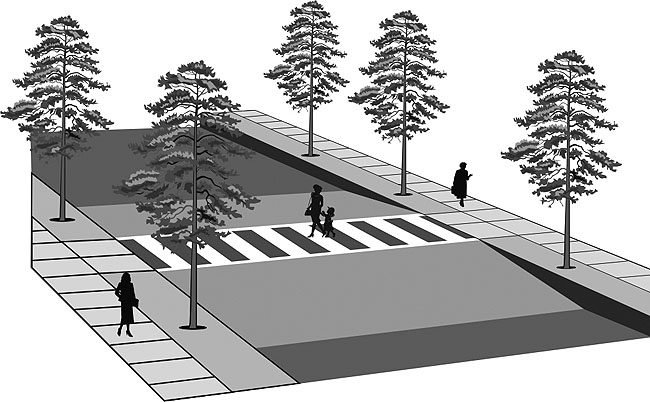
\includegraphics[width=0.7\textwidth]{xwalk.jpg}
	\caption{A raised crosswalk\cite{kimley-xwalk}}\label{fig:xwalk}
\end{figure}

The advantages of such a traffic calming measure include:\begin{itemize}
	\item Forces traffic to slow down, improving pedestrian safety.
	\item Draws attention to the pedestrian, especially when combined with signage and markings.
	\item Makes crossing the street easier for those on wheelchairs.
\end{itemize}

The drawbacks are:\begin{itemize}
	\item The textured materials used tend to be expensive.
	\item Not suitable for emergency or bus routes.
	\item Drainage, especially in snowy or rainy areas, requires additional management.
\end{itemize}


Raised crosswalks are an effective traffic calming technique in that they can reduce vehicular speed (See Table ~\ref{table:xwalk-speed-reduction}). Further, they have also been shown effective at encouraging pedestrians to use the crosswalk instead of crossing the road elsewhere. One study \cite{pedsafe-xwalks} found that raising the crosswalk increased the percentage of pedestrians using it from 11.5\% to 38.3\%. 

% Please remember to add \use{multirow} to your document preamble in order to suppor multirow cells
% Booktabs require to add \usepackage{booktabs} to your document preamble
\begin{table}[h]
\begin{tabular}{@{}lrrr@{}}
\toprule
\multirow{2}{*}{City and Measure}    & \multicolumn{2}{l}{50th percentile speed (km/h)} & \multirow{2}{*}{Speed reduction (km/hr)} \\ \cmidrule(lr){2-3}
      & Treatment Site           & Control Site          &                  \\ \midrule
\begin{tabular}[l]{@{}l@{}}Durham, NC – Research Drive\\ \textit{Raised crosswalk}\end{tabular}                    & 33.3                     & 39.8                  & 6.5                                      \\
\begin{tabular}[l]{@{}l@{}}Durham, NC – Towerview Drive\\ \textit{Raised crosswalk, overhead flasher}\end{tabular} & 18.5                     & 38.4                  & 19.3                                     \\
\begin{tabular}[l]{@{}l@{}}Montgomery County, MD\\ \textit{Raised Crosswalk}\end{tabular}                          & 34.6                     & 38.6                  & 4.0                                   
\\ \bottomrule
\end{tabular}
\caption{Speed reduction due to raised crosswalks}
\end{table}

According to PEDSAFE \cite{pedsafe-xwalks}, raised crosswalks can mitigate dart-and-dash type incidents in which the driver was unable to see the pedestrian until just before impact. They also prevent vehicles from `trapping' pedestrians. Raised crosswalks are best used in areas of low-volume, low-speed traffic where safety of pedestrians takes a priority, such as residential areas and near schools. As a side benefit, they make crossings much easier for the elderly, the disabled, and the young in these areas.

The cost of such a crosswalk varies from \$2000 to \$15000, with typical cost estimate for one unit being \$4000\cite{traffic-calming-xwalks}. However, this might be significantly increased if a drainage system has to be added.

\begin{figure}[!htbp]
\centering
\begin{subfigure}[t]{0.45\textwidth}
	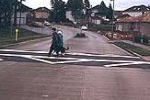
\includegraphics[width=0.9\textwidth]{xwalk1}
	\subcaption{Asphalt and highly-visible paint.}
\end{subfigure}
\begin{subfigure}[t]{0.45\textwidth}
	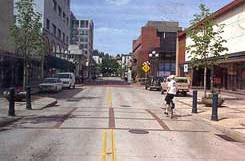
\includegraphics[width=0.9\textwidth]{xwalk2}
	\subcaption{Concrete and brick.}
\end{subfigure}\\
\begin{subfigure}[t]{0.45\textwidth}
	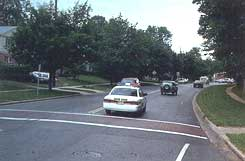
\includegraphics[width=0.9\textwidth]{xwalk3}
	\subcaption{Tapering at the curbs to allow drainage.}
\end{subfigure}
\begin{subfigure}[t]{0.45\textwidth}
	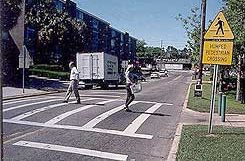
\includegraphics[width=0.9\textwidth]{xwalk4}
	\subcaption{Higher profile crosswalk, almost resembling a speed hump.}
\end{subfigure}
\caption{Various raised crosswalk styles.\cite{traffic-calming-xwalks}}
\end{figure}